\documentclass{article}

% if you need to pass options to natbib, use, e.g.:
%     \PassOptionsToPackage{numbers, compress}{natbib}
% before loading neurips_2020

% ready for submission
% \usepackage{neurips_2020}

% to compile a preprint version, e.g., for submission to arXiv, add add the
% [preprint] option:
%     \usepackage[preprint]{neurips_2020}

% to compile a camera-ready version, add the [final] option, e.g.:
%     \usepackage[final]{neurips_2020}

% to avoid loading the natbib package, add option nonatbib:
     \usepackage[final, nonatbib]{neurips_2020}

\usepackage[utf8]{inputenc} % allow utf-8 input
\usepackage[T1]{fontenc}    % use 8-bit T1 fonts
\usepackage{hyperref}       % hyperlinks
\usepackage{url}            % simple URL typesetting
\usepackage{booktabs}       % professional-quality tables
\usepackage{amsfonts}       % blackboard math symbols
\usepackage{nicefrac}       % compact symbols for 1/2, etc.
\usepackage{microtype}      % microtypography
\usepackage{float}
\usepackage{graphicx}
\usepackage{amsmath}


\title{ECSE 551 Mini Project 1}

% The \author macro works with any number of authors. There are two commands
% used to separate the names and addresses of multiple authors: \And and \AND.
%
% Using \And between authors leaves it to LaTeX to determine where to break the
% lines. Using \AND forces a line break at that point. So, if LaTeX puts 3 of 4
% authors names on the first line, and the last on the second line, try using
% \AND instead of \And before the third author name.

\author{
  Isabel Lougheed,~260989364 \\
  \And
  Mathieu Mailhot,~260989370 \\
  \And
  Frank-Lucas Pantazis,~260986139 \\
  % examples of more authors
  % \And
  % Coauthor \\
  % Affiliation \\
  % Address \\
  % \texttt{email} \\
  % \AND
  % Coauthor \\
  % Affiliation \\
  % Address \\
  % \texttt{email} \\
  % \And
  % Coauthor \\
  % Affiliation \\
  % Address \\
  % \texttt{email} \\
  % \And
  % Coauthor \\
  % Affiliation \\
  % Address \\
  % \texttt{email} \\
}

\makeatletter
\renewcommand{\@noticestring}{}  % Removes footer text
\makeatother

\begin{document}

\maketitle

\begin{abstract}
  This project involves implementing a logistic regression linear classifier from scratch.  This report presents the results of the logistic regression classifier model when performed on two datasets, a Chronic Kidney Disease (CKD) dataset and a battery dataset.  INCLUDE IMPORTANT FINDINGS.
\end{abstract}

\section{Introduction}

\section{Datasets}


The first dataset used is a CKD dataset that is comprised of 28 numerical features which each represent a medical measurement of a patient.  There is one target variable indicating whether the patient was diagnosed with CKD ('CKD') or not diagnosed with CKD ('Normal').  WRITE MORE ABOUT OUR FINDINGS ABOUT THE DATASET.
\\
\\
The second dataset used in this project is a battery dataset comprised of 32 real-valued features which represent specific battery attributes.  There is a target variable to classify whether the battery is normal ('Normal') or defective ('Defective').  WRITE MORE ABOUT OUR FINDINGS ABOUT THE DATASET.


\section{Results}
\subsection{Hyper Parameter Analysis}

\subsection{Linear Model With All Features}

\subsection{Removed Feature Model}

\subsection{Quadratic Model}

One of the models explored in this project is a quadratic model.  This was implemented by adding a quadratic term to the learned function for the more important features, the features with the highest weights attributed to them from the regular linear model.  For the chosen important features $x_i$, 
\begin{equation}
   f_w(x) = w_0 + w_1 x_i + w_2 x_i^2 + \dots
\end{equation}

A cross validation was performed on the quadratic model for each of the datasets for different amounts of quadratic features.  As seen in Figure !!!!, 
as the number of quadratic terms increases, the error increases.  Therefore, for both the CKD quadratic model and the battery quadratic model, only one feature has a quadratic term in the learned function.   
Since the weights of the CKD linear model are 
\begin{equation*}
  \begin{aligned}
    [-1.0179,  2.4871, -0.0185,  0.1225, 0.0509,  0.1222, -0.2118, -0.2312, -0.3058, -0.1395, \\
    0.1897,  0.4275,  0.1648, -0.1032, -0.2050,  0.2870,  0.2827,  0.0557, 0.1185,  0.1652, \\
    -0.0089, -0.3447, -0.2880,  0.0708, 0.0002, -0.0845, -0.0942,  0.1653, -0.7693],
  \end{aligned}
\end{equation*}
the feature that has the largest weight magnitude, excluding  the bias weight is feature 2 and therefore feature 2 has a quadratic term.   
Since the weights of the battery linear model are 
\begin{equation*}
  \begin{aligned}
    [5.5288, 5.4114, -0.0814, 0.0036, 0.0838, -0.3571, -0.9275, -0.8126, -0.2352, -0.0839, \\
    -0.1379, -0.2578, -0.0698, -0.5288, -0.3349, -0.5354, -0.2542, -0.2727, -0.0385, -0.1533, \\
    -0.1472, 0.0454, 0.1609, 0.1094, 0.0360, -0.7155, 0.0190, -0.6298, -0.4767, -0.3815, \\
    -0.3547, -0.3608, -1.6986],
  \end{aligned}
  \end{equation*}
the feature that has the largest weight magnitude, excluding the bias weight is feature 1 and therefore feature 1 has a quadratic term. 

\subsection{Cubic Model}

To further expand the model, a cubic model was also tested.   The implementation of the cubic model is very similar to the quadratic model, except the more important features have polynomial terms of degree three in the learned function.  For the chosen important features $x_i$,
\begin{equation}
  f_w (x) = w_0 + w_1 x_i + w_2 x^2_i + w_3 x^3_i + \dots
\end{equation}
A cross validation was performed on the cubic model for each of the datasets for different amounts of cubic features.  
As seen in Figure !!!, as the number of cubic terms increases, the error increases.  Therefore, for both the CKD cubic model and the battery cubic model, only one feature has a cubic term in the learned function.  
This means that for the CKD cubic model, feature 2 has a cubic term and for the battery cubic model, feature 1 has a cubic term. 

\subsection{Cross Validation}

\begin{table}[h!]
  \centering
  \caption{Cross validation of different CKD models}
  \begin{tabular}{|l|l|l|}
  \hline
  \textbf{CKD Model}                               & \textbf{MSE}                  & \textbf{Error}               \\ \hline
  Linear model with all normalized features        & 0.21073183686528782           & 0.16896551724137931          \\ \hline
  Linear model with all standardized features      & 0.21760510560452745           & 0.1724137931034483           \\ \hline
  Feature removed model                            &             &           \\ \hline
  Quadratic model                                  & 0.20873582936775956           & 0.15862068965517245          \\ \hline
  Cubic model                                      & 0.2078159785211106            & 0.15517241379310348          \\ \hline
  \end{tabular}
\end{table}

\begin{table}[h!]
  \centering
  \caption{Cross validation of different battery models}
  \begin{tabular}{|l|l|l|}
  \hline
  \textbf{Battery Model}                            & \textbf{MSE}                  & \textbf{Error}               \\ \hline
  Linear model with all normalized features         & 0.0886492622549294            & 0.05846153846153843          \\ \hline
  Linear model with all standardized features       & 0.0886183051677138            & 0.05846153846153843          \\ \hline
  Feature removed                                   &            &           \\ \hline
  Quadratic model                                   & 0.08897472474905832           & 0.05846153846153843          \\ \hline
  Cubic model                                       & 0.08894956726027695           & 0.05846153846153843          \\ \hline
  \end{tabular}
\end{table}

\section{Discussion and Conclusion}

\section{Statement of Contributions}

\section{Appendix}

\begin{figure}[H]
  \centering
  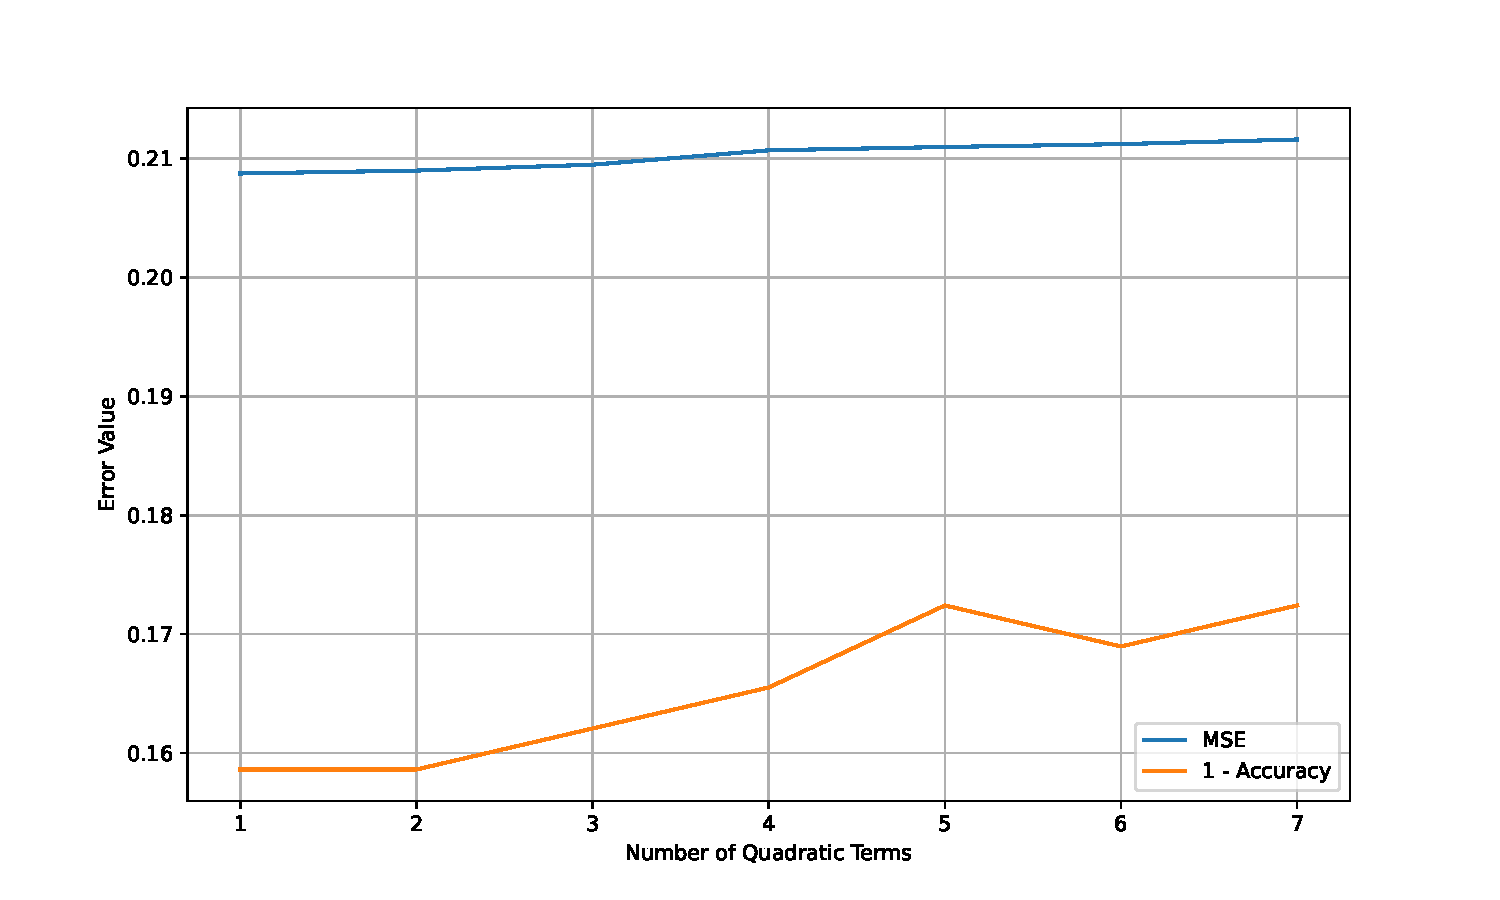
\includegraphics[width=0.8\textwidth]{quad_ckd.pdf}
  \caption{Number of quadratic terms vs. error for the CKD quadratic model}
  \label{fig:quad_ckd}
\end{figure}

\begin{figure}[H]
  \centering
  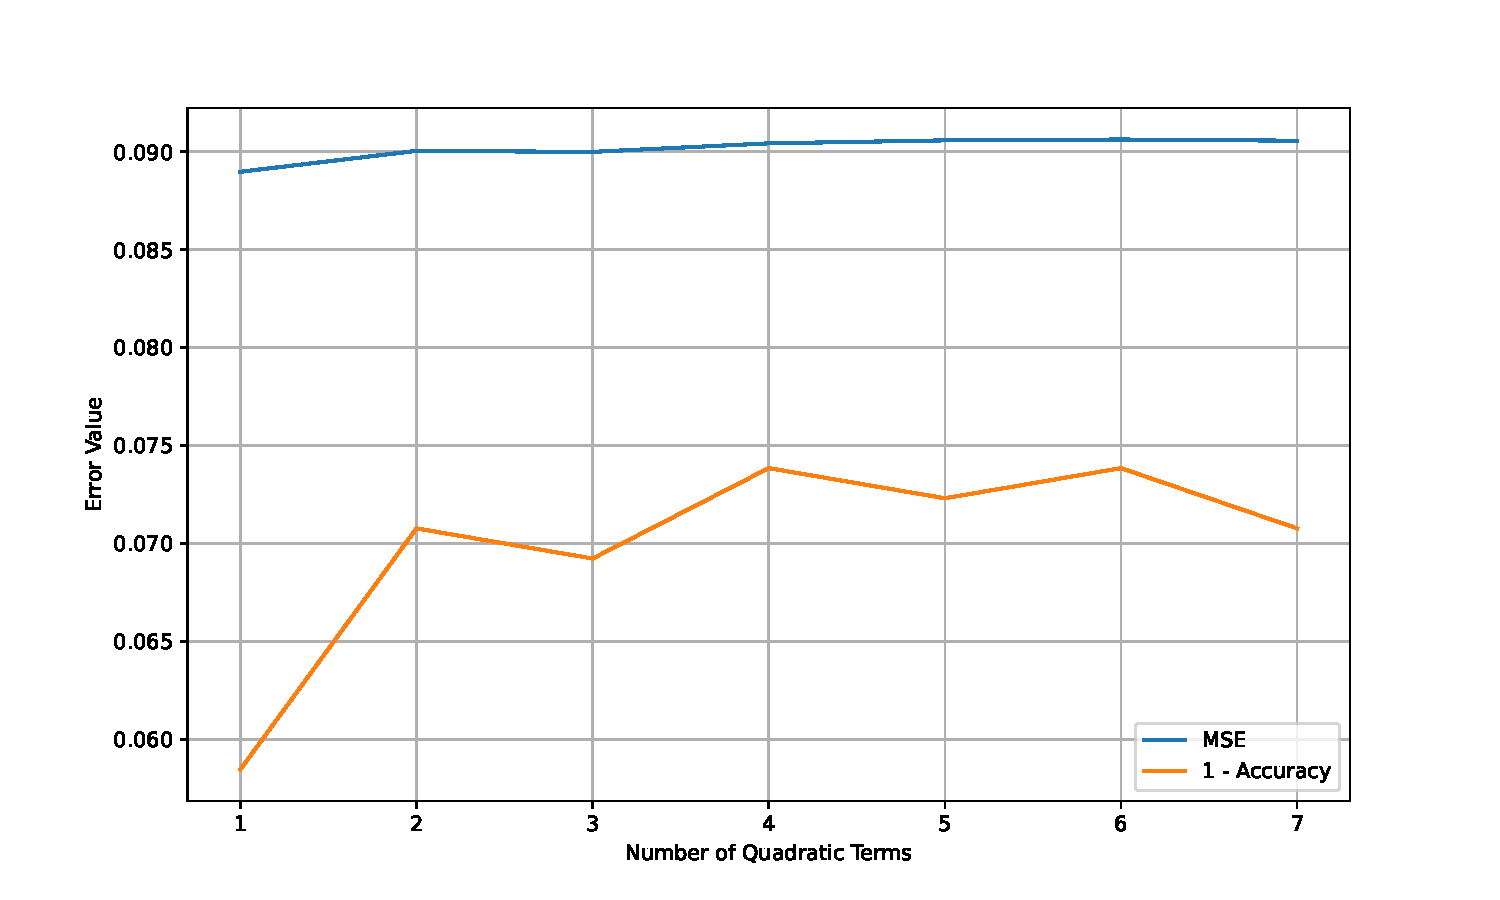
\includegraphics[width=0.8\textwidth]{quad_battery.pdf}
  \caption{Number of quadratic terms vs. error for the battery quadratic model}
  \label{fig:quad_battery}
\end{figure}

\begin{figure}[H]
  \centering
  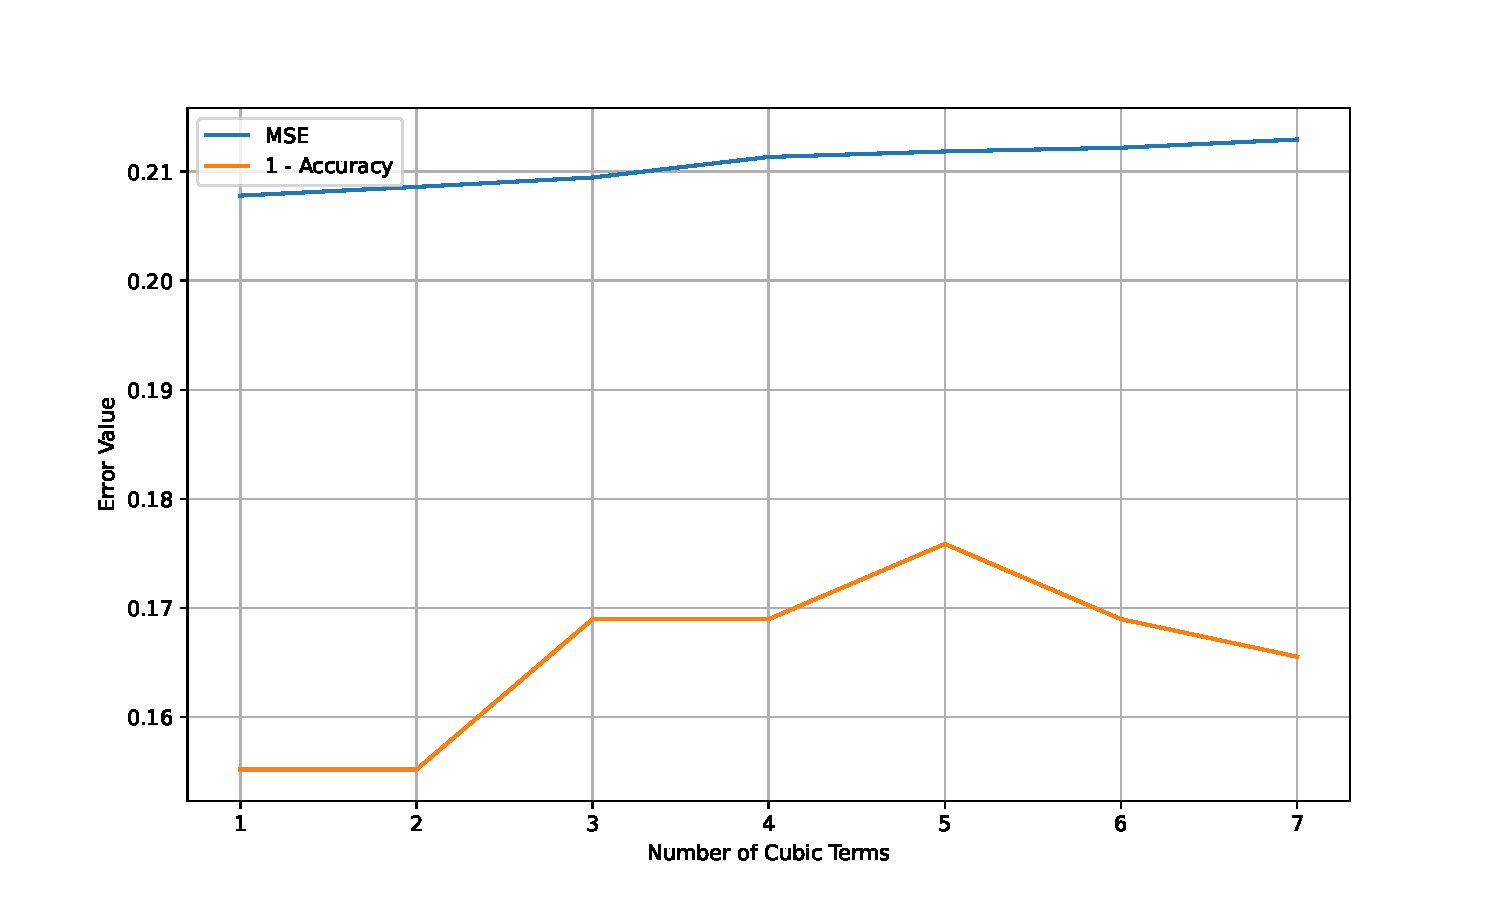
\includegraphics[width=0.8\textwidth]{cubic_ckd.pdf}
  \caption{Number of cubic terms vs. error for the CKD cubic model}
  \label{fig:quad_ckd}
\end{figure}

\begin{figure}[H]
  \centering
  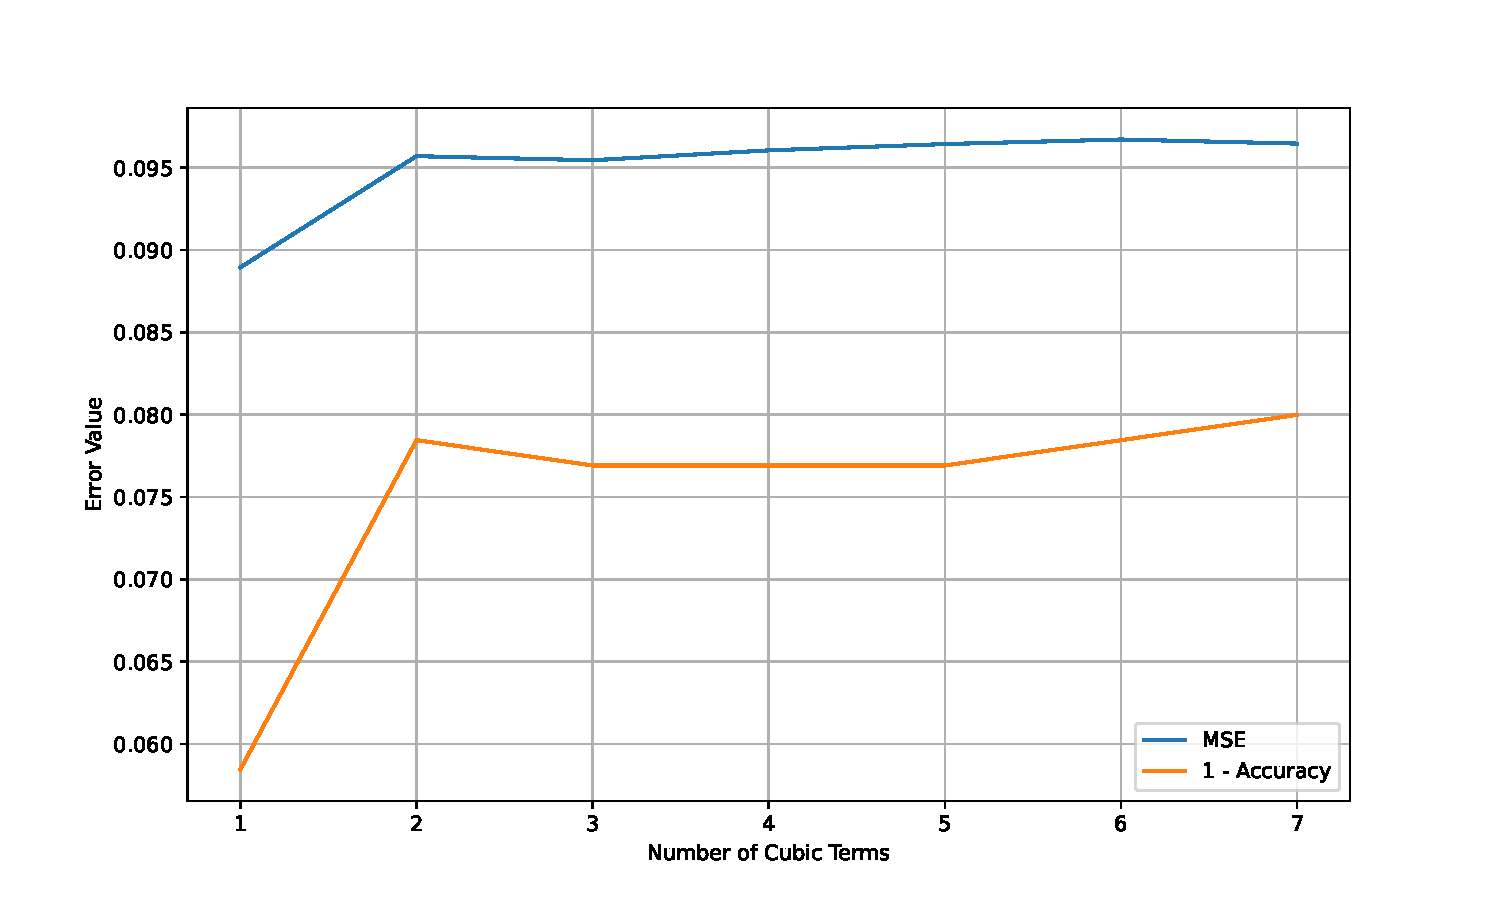
\includegraphics[width=0.8\textwidth]{cubic_battery.pdf}
  \caption{Number of cubic terms vs. error for the battery cubic model}
  \label{fig:quad_battery}
\end{figure}

\section*{References}

References follow the acknowledgments. Use unnumbered first-level heading for
the references. Any choice of citation style is acceptable as long as you are
consistent. It is permissible to reduce the font size to \verb+small+ (9 point)
when listing the references.
{\bf Note that the Reference section does not count towards the eight pages of content that are allowed.}
\medskip

\small

[1] Alexander, J.A.\ \& Mozer, M.C.\ (1995) Template-based algorithms for
connectionist rule extraction. In G.\ Tesauro, D.S.\ Touretzky and T.K.\ Leen
(eds.), {\it Advances in Neural Information Processing Systems 7},
pp.\ 609--616. Cambridge, MA: MIT Press.

[2] Bower, J.M.\ \& Beeman, D.\ (1995) {\it The Book of GENESIS: Exploring
  Realistic Neural Models with the GEneral NEural SImulation System.}  New York:
TELOS/Springer--Verlag.

[3] Hasselmo, M.E., Schnell, E.\ \& Barkai, E.\ (1995) Dynamics of learning and
recall at excitatory recurrent synapses and cholinergic modulation in rat
hippocampal region CA3. {\it Journal of Neuroscience} {\bf 15}(7):5249-5262.

\end{document}